
%% ==================================================================================================
%%
\documentclass[12pt]{book}
\usepackage{amsfonts}
\usepackage{amsmath}
\usepackage{amssymb}
\usepackage{graphicx}
\usepackage{hyperref}
\usepackage{float}
\usepackage{verbatim}
\usepackage{xlop} %% for multiplication https://tex.stackexchange.com/questions/11702/how-to-present-a-vertical-multiplication-addition
\usepackage{listings} %% to format generic computer code
\usepackage{lmodern} % for bold teletype font
\usepackage{minted} % colour Java code

\usepackage{tasks}
%\NewTasks[style=enumerate,counter-format=tsk[A].,label-width=3ex]{choice}[\item](4)

%% =======   set page margins    =======
\setlength{\textheight}{10in}
\setlength{\textwidth}{7.4in}
\setlength{\topmargin}{-0.75in}
\setlength{\oddsidemargin}{-0.5in}
\setlength{\evensidemargin}{-0.5in}
\setlength{\parskip}{0.15in}
\setlength{\parindent}{0in}

%%  for European long division
% https://tex.stackexchange.com/questions/432435/how-to-set-up-european-french-style-long-division-in-tex
\newcommand\frdiv[5]{%
    \[
    \renewcommand\arraystretch{1.5}
    \begin{array}{l| l}
    #1 & #2 \\
    \cline{2-2}
    #3 & #4 \\
    \cline{1-1}
    #5 & \\
    \end{array}
    \]
}

%%  for European long division


%% ==================================================================================================

\begin{document}

%\title{ITI1100 Digital Systems I}
%\author{Kien Do 300163370}
%\date{Assignment \#1}
\newcommand{\reporttitle}{Laboratoire 2}
\newcommand{\reportauthorOne}{Kien Do}
\newcommand{\cidOne}{300163370}
\input{titlePage/titlepage.txt}



%% ==================================================================================================

%%%%%%%%%%%% PROBLEMS START HERE

\begin{enumerate}
\item

    \begin{enumerate}
        \item La dimension de cette pile est 27.
        \item Ce qui arrive à chaque appel de fonction: \\(4), (4, 1), (4, 1, 3), (1, 3), (3), (3, 0), (3, 0, 2), (0, 2), (0, 2, 7), (2, 7), (7)\\
        Les valeurs retournées par la sequence d'opérations sont [4, 1, 3, 0, 2]
        \item  Ce qui arrive à chaque appel de fonction: \\(10), (10, 2), (10, 2, 7), (1, 10, 2, 7), (7), (5, 1, 10, 2, 7), (5, 1, 10, 2), (5, 1, 10, 2, 6), (5, 1, 10, 2, 6, 8), (5), (8), (5, 1, 10, 2, 6, 8, 4), (7)\\
        Les valeurs retournées par la sequence d'opérations sont [7, 7, 5, 8, 7]
        \item Voyez le tableau rempli ci-dessous\\ 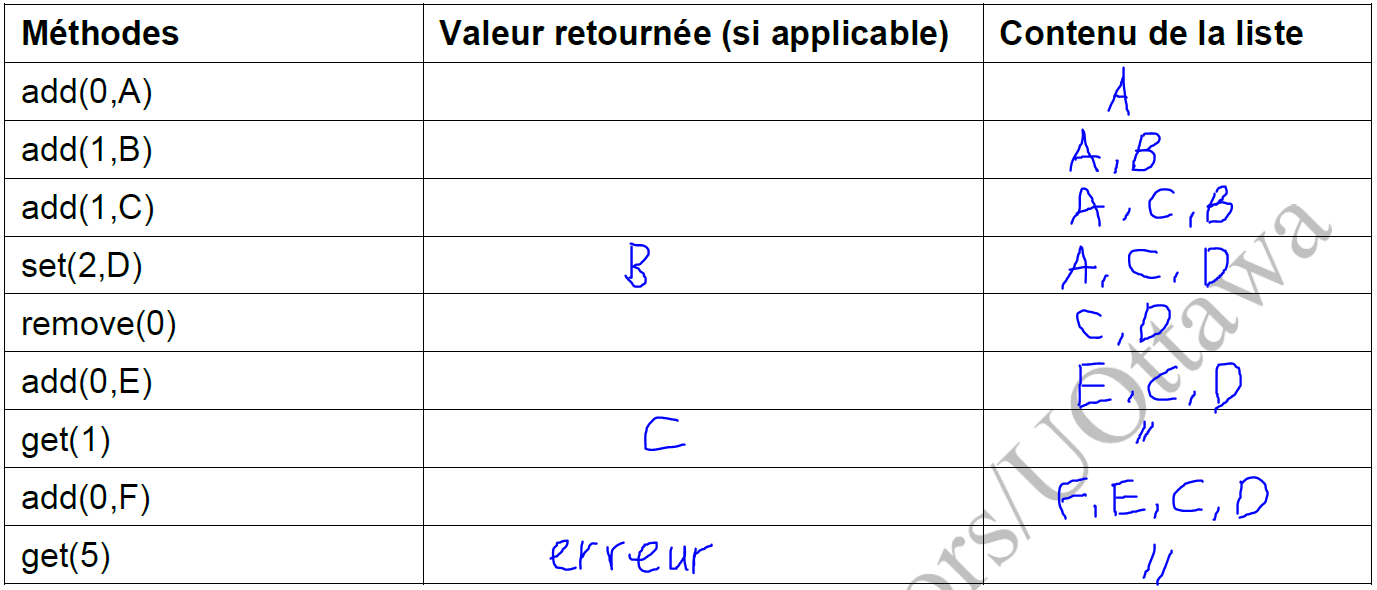
\includegraphics[scale=0.5]{question1d.png}
    \end{enumerate}

\item 
\begin{minted}[breaklines,frame=single]{java}
import java.util.Stack;

/**
 * A Stack that keeps track of the maximum element (the element with the highest integer value)
 */
public class GreatStack extends Stack<Integer> {

    // to keep track of max values
    private Stack<Integer> maxList;

    /**
     * Constructor for GreatStack
     */
    public GreatStack() {
        // instantiate a maxList for every GreatStack created
        maxList = new Stack<Integer>();
    }

    /**
     * Used by pushh() to add the new pushed value to the maxList to keep track of the max value
     * @param num
     */
    private void addToMaxList(int num) {
        if (maxList.size() == 0) {
            maxList.add(num);
        }
        if (num > maxList.peek()) {
            maxList.push(num);
        } else {
            maxList.push(maxList.peek());
        }
    }

    /**
     * Used by popp() to remove the popped value to the maxList to keep track of the max value
     * @param num
     * Number to be removed from maxList
     */
    private void removeFromMaxList(int num) {
        maxList.pop();
    }

    /**
     * Custom version of .push()
     * @param num
     * Number to be added to maxList
     */
    private void pushh(int num) {
        this.push(num);
        addToMaxList(num);
    }

    /**
     * Custom version of .pop()
     */
    private void popp() {
        removeFromMaxList(this.pop());
    }

    /**
     * Returns the max value of GreatStack
     * @return max
     */
    private int getMax() {
        return maxList.peek();
    }
}


\end{minted}

\newpage
Voici le test\\\\ 
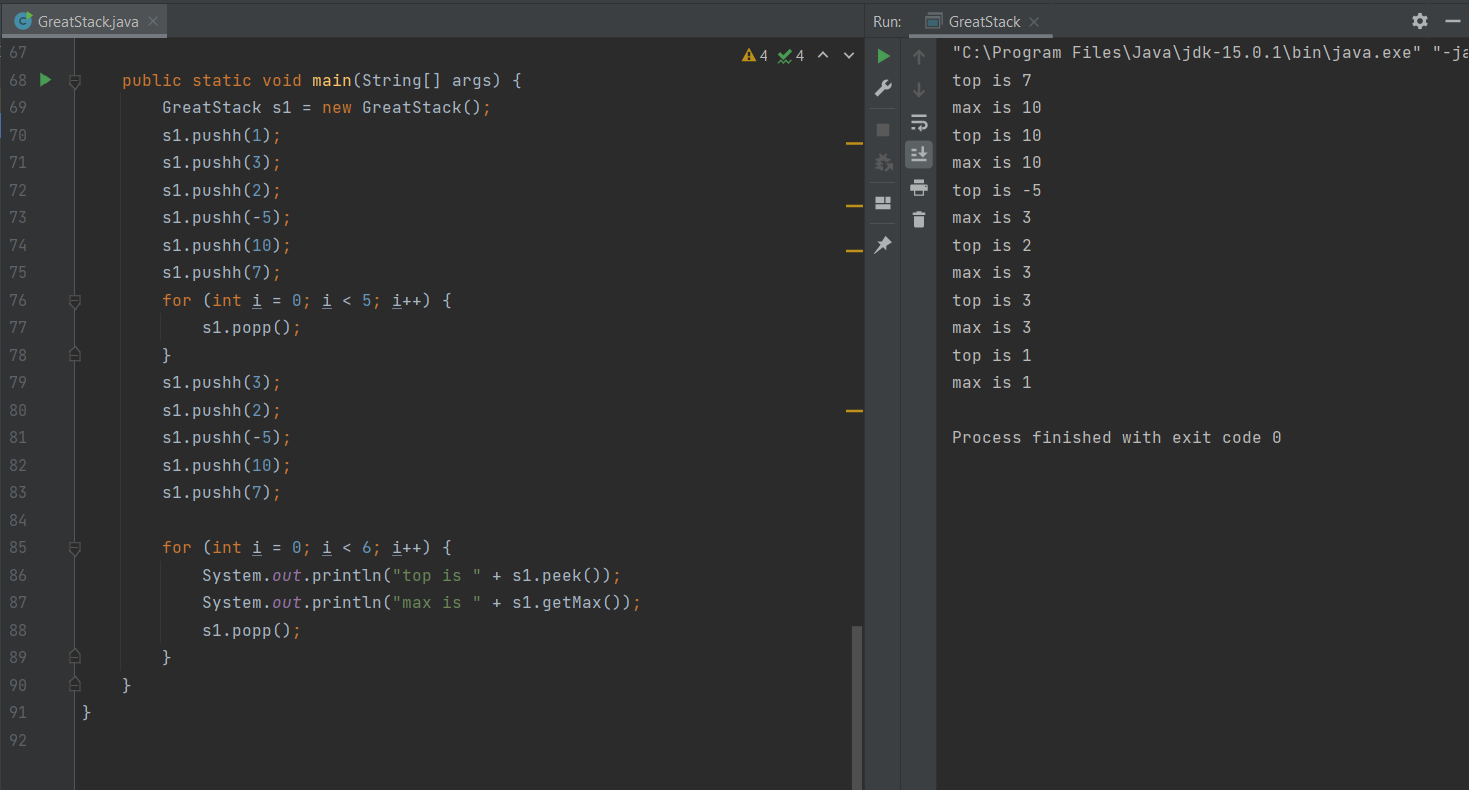
\includegraphics[scale=0.6]{question2test.png}


\end{enumerate}






\end{document} 
